\documentclass[11pt, a4paper]{article}[]
	\usepackage[czech]{babel}
	\usepackage[utf8]{inputenc}
	\usepackage[left=2cm,text={17cm, 24cm},top=3cm, includefoot]{geometry}
	\usepackage{times}

	\usepackage{setspace}	


	\usepackage{graphicx}

	\usepackage{lscape}


\begin{document}

	% titulni strana, opticky stred stranky
	\thispagestyle{empty}

	\begin{center}
		\Huge
			\textsc{Vysoké učení technické v~Brně\\}
		\huge
			\textsc{Fakulta informačních technologií\\}
		\vspace{\stretch{0.382}}
		\LARGE
			IDS - Databázové systémy \\
		\Huge
			Datový model (ERD) a model případů užití \\
		
		\LARGE	zadání projektu\\
			Restaurace \\
		\vspace{\stretch{0.618}}
	\end{center}
		{\Large 23.02.2017 \hfill Miroslava Míšová, Jiří Matějka} % lze pouzit i \today


	\pagebreak  % konec stranky
	\setcounter{page}{1}  % cislovani stranek bude az od druhe strany, kde bude cislo stranky 1


	\section{Zadání}
	Vytvořte IS pro restaurační zařízení, který napomůže k zjednodušení a zpřehlednění jeho provozu. Restaurace je členěna do více místností a má přední a zadní zahrádku a poskytuje běžné stravovací služby veřejnosti. Od informačního systému se požaduje, aby, krom jiného, umožnil správu rezervací a objednávek. Rezervovat je možné jeden nebo více stolů v místnostech či na zahrádkách, anebo celé místnosti, případně i celou restauraci pro různé společenské akce. Součástí rezervace také může být objednávka nápojů a jídel. Systém musí umožňovat zaměstnancům restaurace vkládat objednávky spolu s informacemi, který zaměstnanec danou objednávku vložil a pro koho je určena. Když se zákazníci rozhodnou zaplatit, musí jim systém vystavit účtenku. Po zaplacení pak příslušný zaměstnanec vloží záznam o platbě do systému. Systém by měl také poskytovat podrobný přehled tržeb za vybrané období. Přístup k této funkci bude mít pouze majitel. V neposlední řadě musí systém evidovat veškeré prodávané jídlo a pití (včetně složení), přičemž majitel a odpovědný vedoucí mají možnost měnit ceny jídla a pití nebo přidávat a odebírat položky. 
	

	\section{Use-case diagram}  

	\begin{figure}[h]
	\begin{center} 
		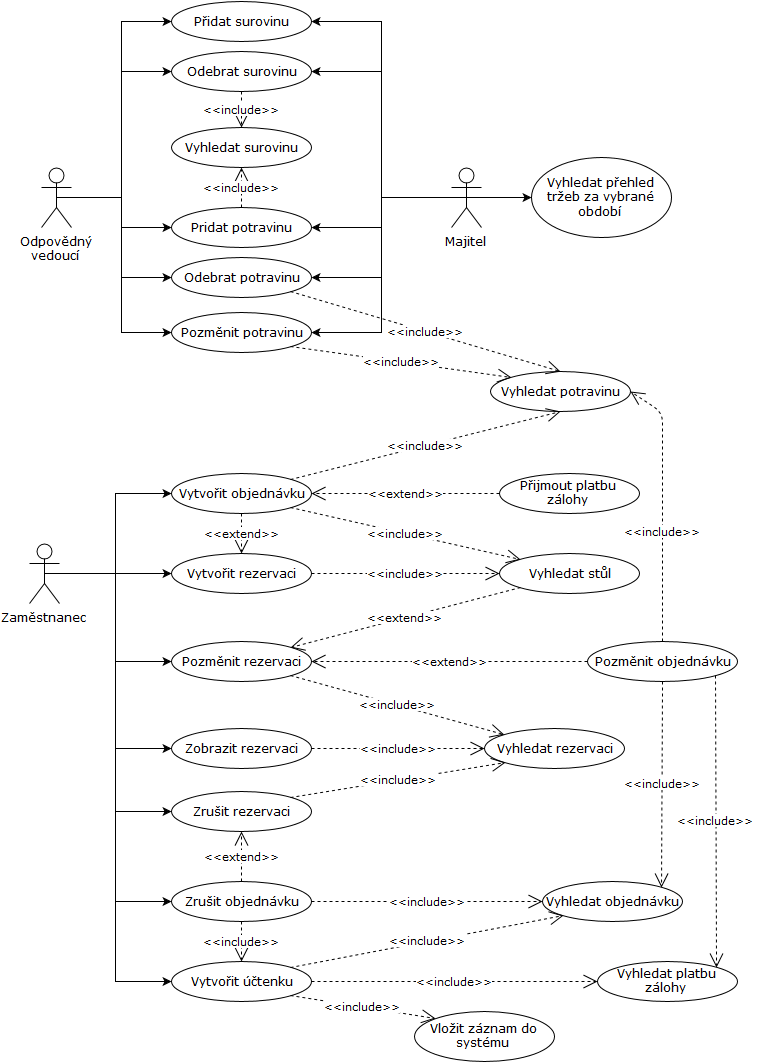
\includegraphics[height=15cm]{use-case.png} 
		\label{fig:obr_use-case}
	\end{center}
	\end{figure}

	\pagebreak  % konec stranky

	
	\section{ER diagram}

	\begin{figure}[h]
	\begin{center} 
		\includegraphics[height=20cm]{ERD.png} 
		\label{fig:obr_ERD}
	\end{center}
	\end{figure}

	

\end{document}
